\documentclass[a4paper]{article}

% Global layout
\usepackage{fancyhdr, graphicx, hyperref, indentfirst, lastpage, setspace}
\usepackage[margin=40mm]{geometry}

% Encoding
\usepackage[utf8]{vntex, inputenc}
\usepackage[english]{babel}
\usepackage{amsmath, amssymb, gensymb}

% Better table
\usepackage{array, booktabs, multicol, multirow, siunitx, tabularx}

% Code space
\usepackage[dvipsnames]{xcolor}
\usepackage{tikz}
\usepackage[framemethod=tikz]{mdframed}
\usepackage{minted, verbatim} % needs --shell-escape flag and Pygments

% Graphics
\usepackage{caption, float}

% Page setup
\allowdisplaybreaks{} % to have page breaks inside align* environment
\hypersetup{urlcolor=blue,linkcolor=black,citecolor=red,colorlinks=true}
\usemintedstyle{emacs}
\numberwithin{equation}{section}
\renewcommand{\arraystretch}{1.2} % space between table rows

% Global style setup
\makeatletter % change font size for not having underfull hbox
\renewcommand\Huge{\@setfontsize\Huge{22pt}{18}}
\makeatother

\AtBeginDocument{\renewcommand*\contentsname{Contents}}
\AtBeginDocument{\renewcommand*\refname{References}}
%\usepackage{fancyhdr}
\setlength{\headheight}{40pt}
\pagestyle{fancy}
\fancyhead{} % clear all header fields
\fancyhead[L]{
  \begin{tabular}{rl}
    \begin{picture}(25,15)(0,0)
      \put(0,-8){
\includegraphics[width=8mm, height=8mm]{./assets/hcmut.png}}
    \end{picture}
    \begin{tabular}{l}
      \textbf{\bf \ttfamily University of Technology, Ho Chi Minh City}\\
      \textbf{\bf \ttfamily Faculty of Computer Science and Engineering}
    \end{tabular}
  \end{tabular}
}
\fancyhead[R]{
	\begin{tabular}{l}
		\tiny \bf \
		\tiny \bf
	\end{tabular}  }
\fancyfoot{} % clear all footer fields
%\fancyfoot[L]{\scriptsize \ttfamily Assignment for Operating system - Academic year 2020 - 2021}
\fancyfoot[R]{\scriptsize \ttfamily Page {\thepage}/\pageref{LastPage}}
\renewcommand{\headrulewidth}{0.3pt}
\renewcommand{\footrulewidth}{0.3pt}

%%%
\setcounter{secnumdepth}{4}
\setcounter{tocdepth}{3}
\makeatletter
\newcounter{subsubsubsection}[subsubsection]
\renewcommand\thesubsubsubsection{\thesubsubsection.\@alph\c@subsubsubsection}
\newcommand\subsubsubsection{\@startsection{subsubsubsection}{4}{\z@}%
                                     {-3.25ex\@plus% -1ex \@minus% -.2ex}%
                                     {1.5ex \@plus% .2ex}%
                                     {\normalfont\normalsize\bfseries}}}}
\newcommand*\l@subsubsubsection{\@dottedtocline{3}{10.0em}{4.1em}}
\newcommand*{\subsubsubsectionmark}[1]{}
\makeatother

\setlength{\parindent}{1em}
\setlength{\parskip}{1em}
%\doublespacing
\begin{document}

\begin{titlepage}
  \begin{center}
    VIETNAM NATIONAL UNIVERSITY, HO CHI MINH CITY \
    UNIVERSITY OF TECHNOLOGY \
    FACULTY OF COMPUTER SCIENCE AND ENGINEERING
  \end{center}

  \vspace{1cm}

  \begin{figure}[H]
    \begin{center}
      
\includegraphics[width=4.5cm]{./assets/hcmut.png}
    \end{center}
  \end{figure}

  \vspace{1cm}

    \begin{center}
      \addtolength{\leftskip}{-0.3\textwidth}
      \addtolength{\rightskip}{-0.3\textwidth}
      \begin{tabular}{c}
        \textbf{\Large DATABASE SYSTEMS LAB (CO2014)} \\
        {}                                            \\
        \midrule                                      \\
        \textbf{\Large Assignment 1 Report}           \\
        {}                                            \\
        \textbf{\Huge HOSPITAL MANAGEMENT SYSTEM}
        {}                                            \\
        \bottomrule
      \end{tabular}
    \end{center}

  \vspace{2cm}

  \begin{table}[h]
    \begin{tabular}{rll}
      \hspace{5cm} Advisor:  & Dr.\ Trần Minh Quang           \\
                             &                                \\
      \hspace{5cm} Class:    & CC08                           \\
      \hspace{5cm} Students: & Nguyễn Hoàng         & 1952255 \\
                             & Cao Bá Huy           & 1952713 \\
                             & Lưu Chấn Hưng        & 1952063
    \end{tabular}
  \end{table}

  \begin{center}
    {\footnotesize \large HO CHI MINH CITY, OCTOBER 2021}
  \end{center}
\end{titlepage}

%\thispagestyle{empty}

\newpage
\tableofcontents
\newpage


\section{Requirement description}
\begin{comment}
\subsection{Introduction}
In this assignment, we will demonstrate the process of creating a conceptual design, logical design using relational model and implementing a database using a particular database management system (DBMS) for the hospital management system.
We will carry on step-by-step from describing the requirements to logical designing and lastly, to the implementation.

\subsection{Requirement description}
\end{comment}

In this hospital management database, we will store information about patient medical records.
A PATIENT RECORD should contain a unique record number, the patient's first name and last name, gender, home address, day of birth, diagnosis, treatments, medical background and patientID\@.
In this database, we consider a PATIENT as a RECORD to reduce the complexity, which means a record contains all the individual information of a patient and can be considered a patient also.

Secondly, we store the information about the hospital employees.
An EMPLOYEE should have some basic attributes like: a unique EmployeeID, name, gender, day of birth, job type and salary.
We assume there are 5 types of employees in this hospital which are: Doctor, Nurse, Receptionist, Technician and Driver.
Each of them will inherit all the basic attributes above from the superclass Employee.
Furthermore, each of them will have their own attributes and functionalities like:
\begin{itemize}
  \item  A DOCTOR should have a unique medical practising certificate id, medical degree, experience and specialty.
        A doctor will treat and be responsible for the treatment of multiple patients.
        The treatment start and end dates are also recorded.
        A patient can only have one doctor treating at one department to reduce complexity.

        We also store the department where each doctor belongs.
        A department will have a unique name, unique id and location.
        Moreover, a department will consist of many rooms where the patients stay in and a room can contain many patients.
        We will store some information about each room like room ID (unique), the number of beds left and room type.
        We also record the bed that a patient use, the dates where a patient uses the bed and leaves.

  \item A NURSE will have a medical degree and experience recorded in the system.
        A nurse can take care of multiple patients.

  \item A RECEPTIONIST will arrange the meeting between the patient and the doctor by maintaining an appointment record.
        An appointment record should have a unique id, date and time.
        Furthermore, patients can have many appointment records because they may want to consult with other doctors in different departments.

  \item A TECHNICIAN will have his/her own specialty such as: computer, electrical, thermal engineering, etc\@.
        A technician will manage many equipment that are installed in each room of each department.
        Additionally, we also store the data about the equipment like the unique equipment id, the type, bought date and the maintenance date.

  \item A DRIVER will have a unique license id and can only use 1 ambulance to transport the patients.
        The ambulance's number and license plate are also recorded.
\end{itemize}

Finally, information about the treatment of patients are recorded:
\begin{itemize}
  \item A patient may have many medical PRESCRIPTIONS which include an id (unique) and the date.
        Each prescription can have many types of medicine and vice versa.
        A type of MEDICINE may have some information like ID (unique), brand name, generic name and manual description.
        Dose of each prescription shall be recorded.

  \item Patients will have their own PAYMENT and this information should be stored.
        A PAYMENT will include a unique id, amount, method and date.

  \item We also save the TREATMENT that is provided for each patient record, a TREATMENT will have a treatment id (unique), treatment name, requirement and description.
        The date that the treatment is taken should be also saved.

  \item In order to indicate the problem a patient is having, the patient has to take one or many diagnostic tests.
        Data about the TEST such as the unique test id, test name and description should be collected.
        Additionally, the date and the result of the test are recorded too.
\end{itemize}

\newpage

\section{Conceptual design with ER diagram}
From the requirement description, we obtain the following ER diagram.

\begin{figure}[H]
  \centering
  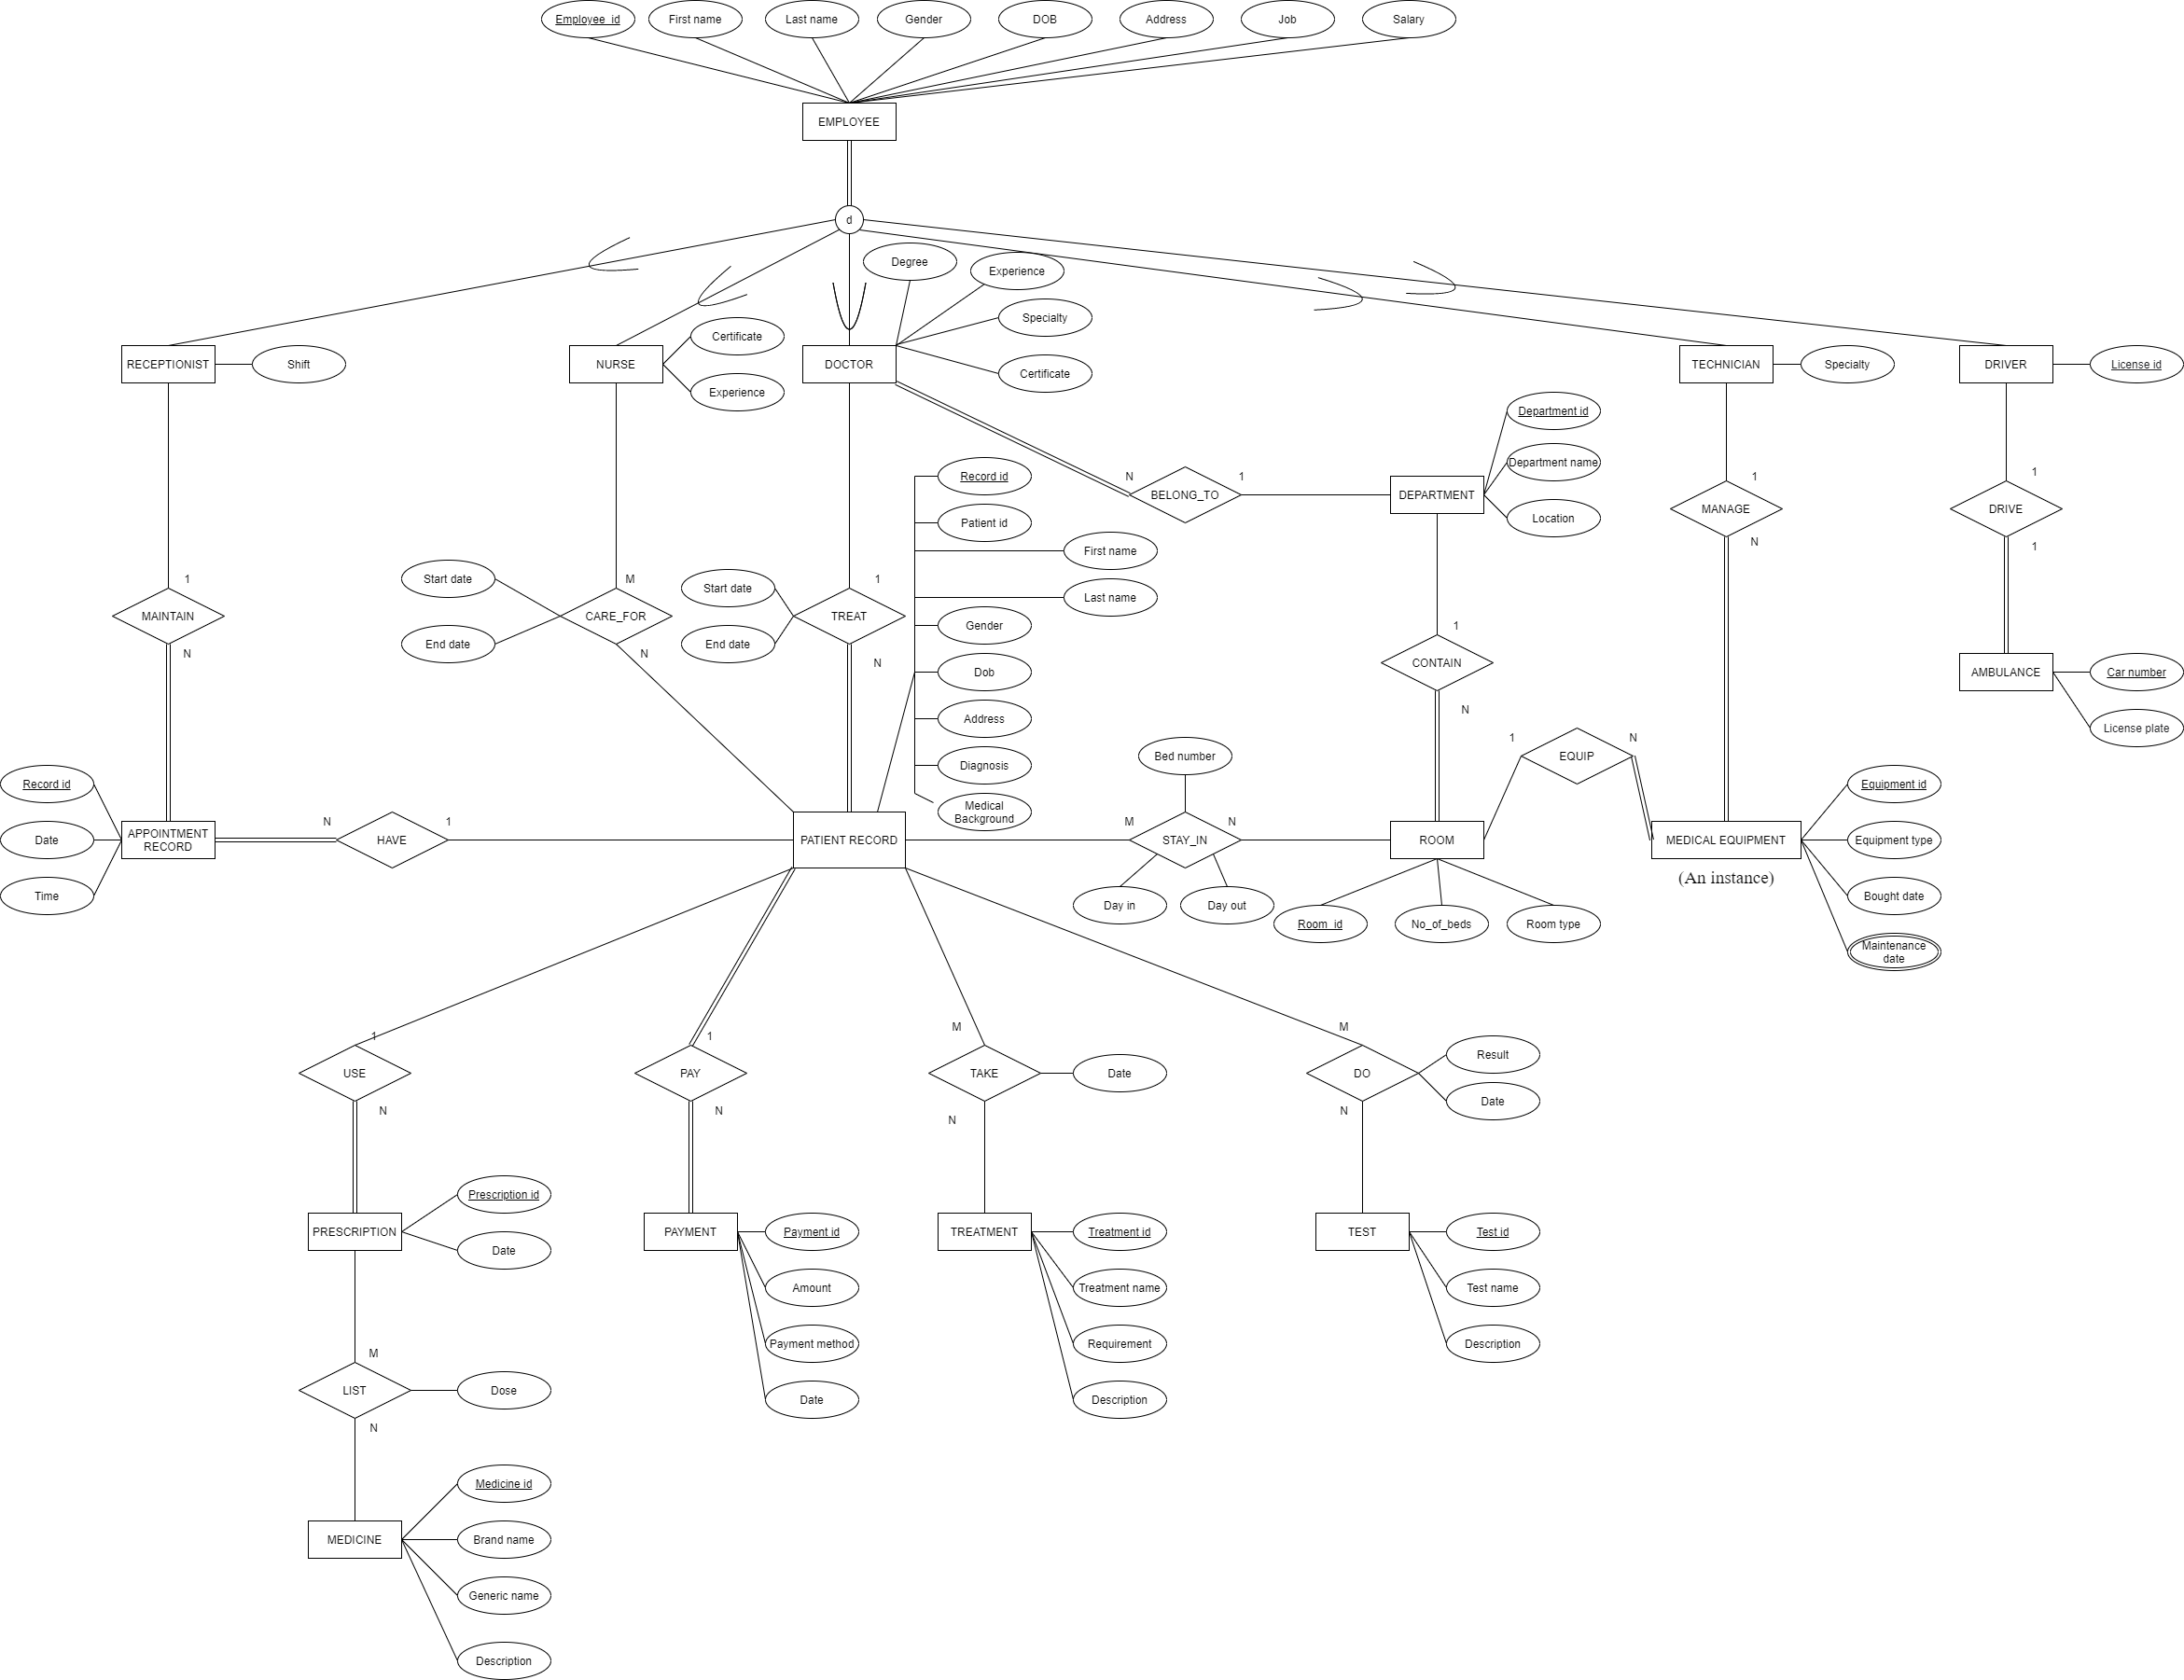
\includegraphics[width=0.9\textwidth]{./assets/erd.png}\label{ER diagram of hospital management system}
\end{figure}

You can find a high quality version of this figure at \url{https://i.imgur.com/2gl84iB.png}.

\newpage

\section{Logical design}
From the requirement description, we obtain the following ER diagram.

\begin{figure}[H]
  \centering
  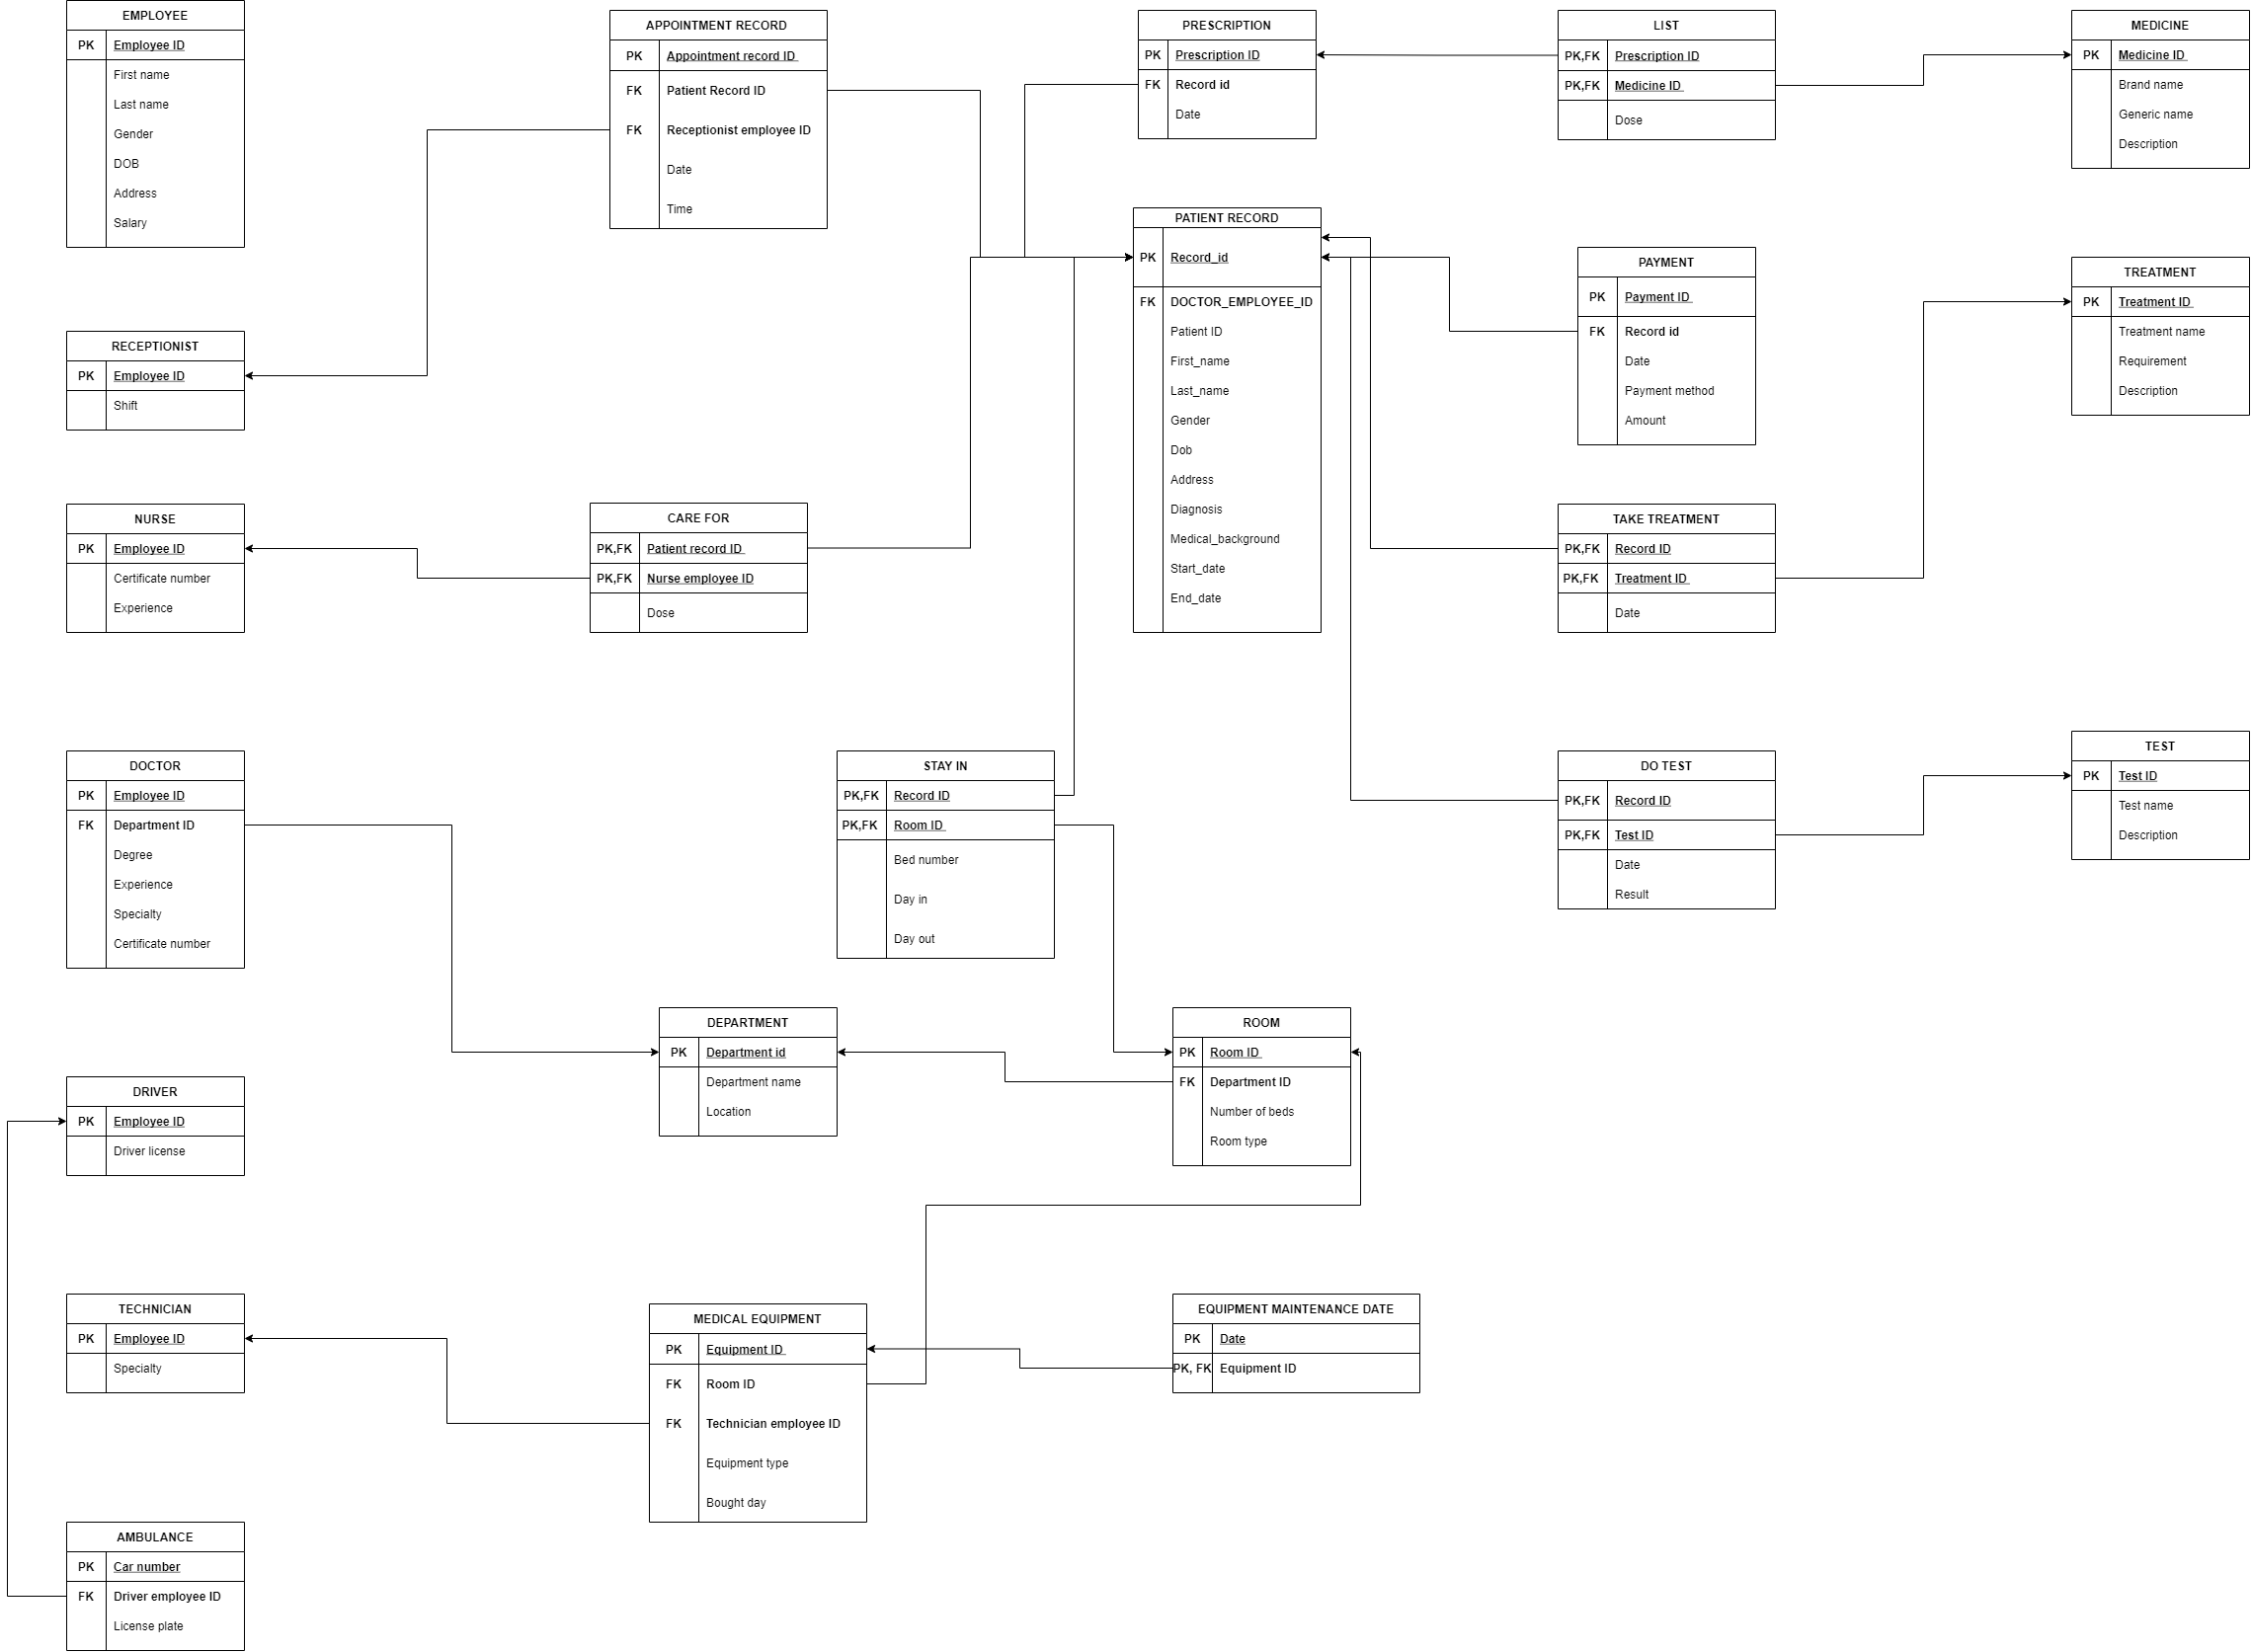
\includegraphics[width=0.9\textwidth]{logical design.png}\label{Logical design}
\end{figure}

You can find a high quality version of this figure at \url{https://i.imgur.com/iNemgZS.png}.

\newpage



\section{Using MySQL Workbench for designing relational model.}
\subsection{Introduction to MySQL Workbench}
% MySQL is an open-source relational database management (RDBMS) system that works on many platforms.
% It allows multi-user access while supporting many storage engines and is backed by Oracle.
% Like the name suggests MySQL is based structured query language (SQL).

% MySQL operates using client/server architecture in which the server runs on the machine containing the databases and clients connect to the server over a network.
% Typically MySQL is supported on Windows XP, Windows Server 2003, Red Hat Fedora Linux, and Debian Linux, and many more.
% As with any other client/server application, MySQL is a multi-user database system, meaning several users can access the database simultaneously.

\begin{itemize}
    \item MySQL Workbench is a Visual database designing and modeling access tool for MySQL server relational database.
    \item The purpose of MySQL workbench is to provide the interface to work with databases more easily and in a more structured way.
    \item It facilitates creation of new physical data models and modification of existing MySQL databases with reverse/forward engineering and change management functions. 
\end{itemize}

\subsection{Pros}
\begin{itemize}
    \item MySQL workbench is GUI for MySQL, which is the most popula DBMS.
\item MySQL workbench has a free (community) version
\item Huge amount of resources and features . For example : Reverse engineering , forward engineering , data migration, ...
\item Reverse and forward engineering make the database design process easy to perform. % t tính để cái đó dô pro, con thôi , khỏi feature 
\end{itemize}
% Rev & forw engineering cho vào feature ↓

\subsection{Cons}
\begin{itemize}
    \item Only works for MySQL.
\item Does not support collaboration.
\item Some features are available only in paid versions.
\item It is quite complicated and overkill to perform simple tasks.
\end{itemize}

\newpage

%----------------------------------------------%

\section{Our choice of DBMS: MySQL }
\subsection{Some main features of MySQL}
\subsubsection{Data types}
        MySQL supports a variety of data types: signed and unsigned integers; 1, 2, 3, 4, and 8 bytes long FLOAT, DOUBLE; CHAR, VARCHAR,\dots
        MySQL also supports time data.
        For example: DATE, TIME, CHAR(n)\dots

\subsubsection{MySQL is open-source}
        Any individual or enterprise may freely use, modify, publish, and expand on Oracle’s open-source MySQL code base.
        The software is released under the GNU General Public License (GPL).

        For MySQL code to be integrated or included in a commercial application (or if open-source software is not a priority), enterprises can purchase a commercially licensed version from Oracle.

\subsubsection{Security}
        A privilege and password system that is very flexible and secure, and makes sure that only authorized users have access to the database.
        Password security by encryption of all password traffic when you connect to a server.

\subsubsection{Compatible on many operating systems}

MySQL is compatible to run on many operating systems, like Novell NetWare, Windows, Linux, many varieties of UNIX (such as Sun Solaris, AIX, and DEC UNIX), OS/2, FreeBSD, and others. MySQL also provides a facility that the clients can run on the same computer as the server or on another computer (communication via a local network or the Internet).

\subsubsection{GUI Support}

MySQL provides a unified visual database graphical user interface tool named  "MySQL Workbench" to work with database architects, developers, and Database Administrators. MySQL Workbench provides SQL development, data modeling, data migration, and comprehensive administration tools for server configuration, user administration, backup, and many more. MySQL has a fully GUI supports from MySQL Server version 5.6 and higher.


\subsection{Why we choose MySQL}
\begin{itemize}
  \item Our hospital management database is a relational database which describes the information and relationships between many tables (entities) so MySQL will be a good choice since this DBMS supports the management of relational database.
  \item MySQL contains records in multiple, separate, and highly codified tables which allows it to optimize actions like data retrieval, updating information, or more complex actions like aggregations better.
  \item The software is easy to install and also uses an event scheduler to schedule the tasks automatically.
  \item MySQL is designed to meet even the most demanding applications while ensuring optimal speed, full-text indexes and unique memory caches for enhanced performance.
\end{itemize}

\newpage

\section{Physical design and Implementation}
\subsection{Physical design}
Previously, we have implemented a logical design for a database, and now we will implement the physical design by adding the datatype for each attribute.

Lets take the patient record as the illustration.

For the sake of simplicity, we decided that all IDs shall be integers, hence the following fields will be assigned INT:
\begin{itemize}
    \item Record\_id
    \item Patient\_id
    \item DOCTOR\_employee\_id
\end{itemize}

A patient record contains some information about time, hence the following fields are assigned DATETIME:
\begin{itemize}
    \item Dob
    \item Start\_date
    \item End\_date
\end{itemize}

Our record also contains information like names, which can only be stored as strings. MySQL does not have an actual string, so we used VARCHAR instead.
We decided that 45 characters is sufficient, hence we use VARCHAR\(45\) for these fields:
\begin{itemize}
    \item First\_name
    \item Last\_name
    \item Address
    \item Diagnosis
    \item Medical\_background
\end{itemize}

And the last field is Gender.
Originally, we wanted this to be a bool, but MySQL does not define such datatype, so we use TINYINT instead.

\begin{comment}%%%%%%%%%%%%
A patient record will have:
\begin{itemize}
    \item Record ID: Each record will have a unique ID to identify, hence we will set this attribute as the key attribute.
    To make things simple, we will assume that a record ID will be an Integer value. 
    
    \item Patient ID: Similar to the Record ID, Patient ID will also be represented by an Integer value. 
    
    \item First name, Last name: In order to record the patient name, we need to have a string to store the name.
    Therefore, we will set the datatype for each of them as VARCHAR(45) which is an array of maximum 45 characters.
    
    \item Gender: To illustrate the gender, we decided to use the BOOLEAN type. A value ``TRUE'' is set if the gender is ``MALE'' , a value ``FALSE'' is set if the gender is ``FEMALE''. 
    
    \item Day of birth: Obviously for date, we have to use the datatype ``Date''. 
    
    \item Address: To store the address of the patient, an array of 45 characters shall be used (VARCHAR(45)). 
    
    \item Diagnosis : This attribute represents the note of the doctor for the patient's disease and condition. Therefore, we will use VARCHAR(45) again. 
    
    \item Medical background : Similar to the diagnosis, we will use VARCHAR(45) to show the medical background of a patient. 
    
    \item Start date , End date : It is obvious that the date the patient was hospitalized and  the date the patient was out of the hospital will be assigned the Date datatype. 
    
    \item Doctor ID : Like the patient ID, the doctor employee ID will be illustrated by an Integer value. 

    
\end{itemize}
\end{comment}%%%%%%%%%%%
    The following picture will show the physical design of the MEDICAL RECORD. 
    
    \begin{center}
        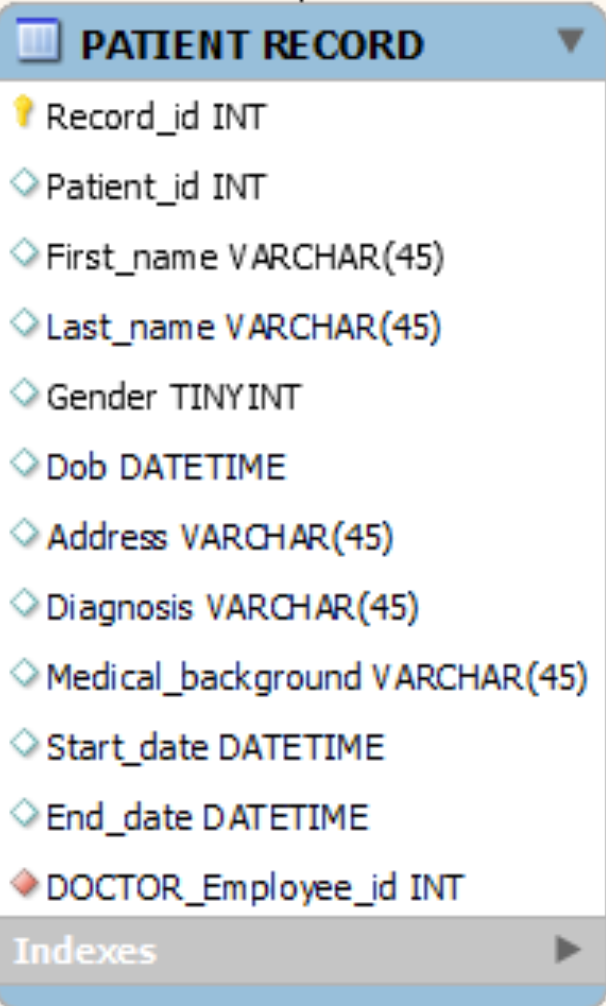
\includegraphics[width=0.3\textwidth]{assets/physical_ex.PNG}
    \end{center}

We repeat this process for all the tables in our logical design and eventually we obtain the following physical design. 

\begin{figure}[H]
  \centering
  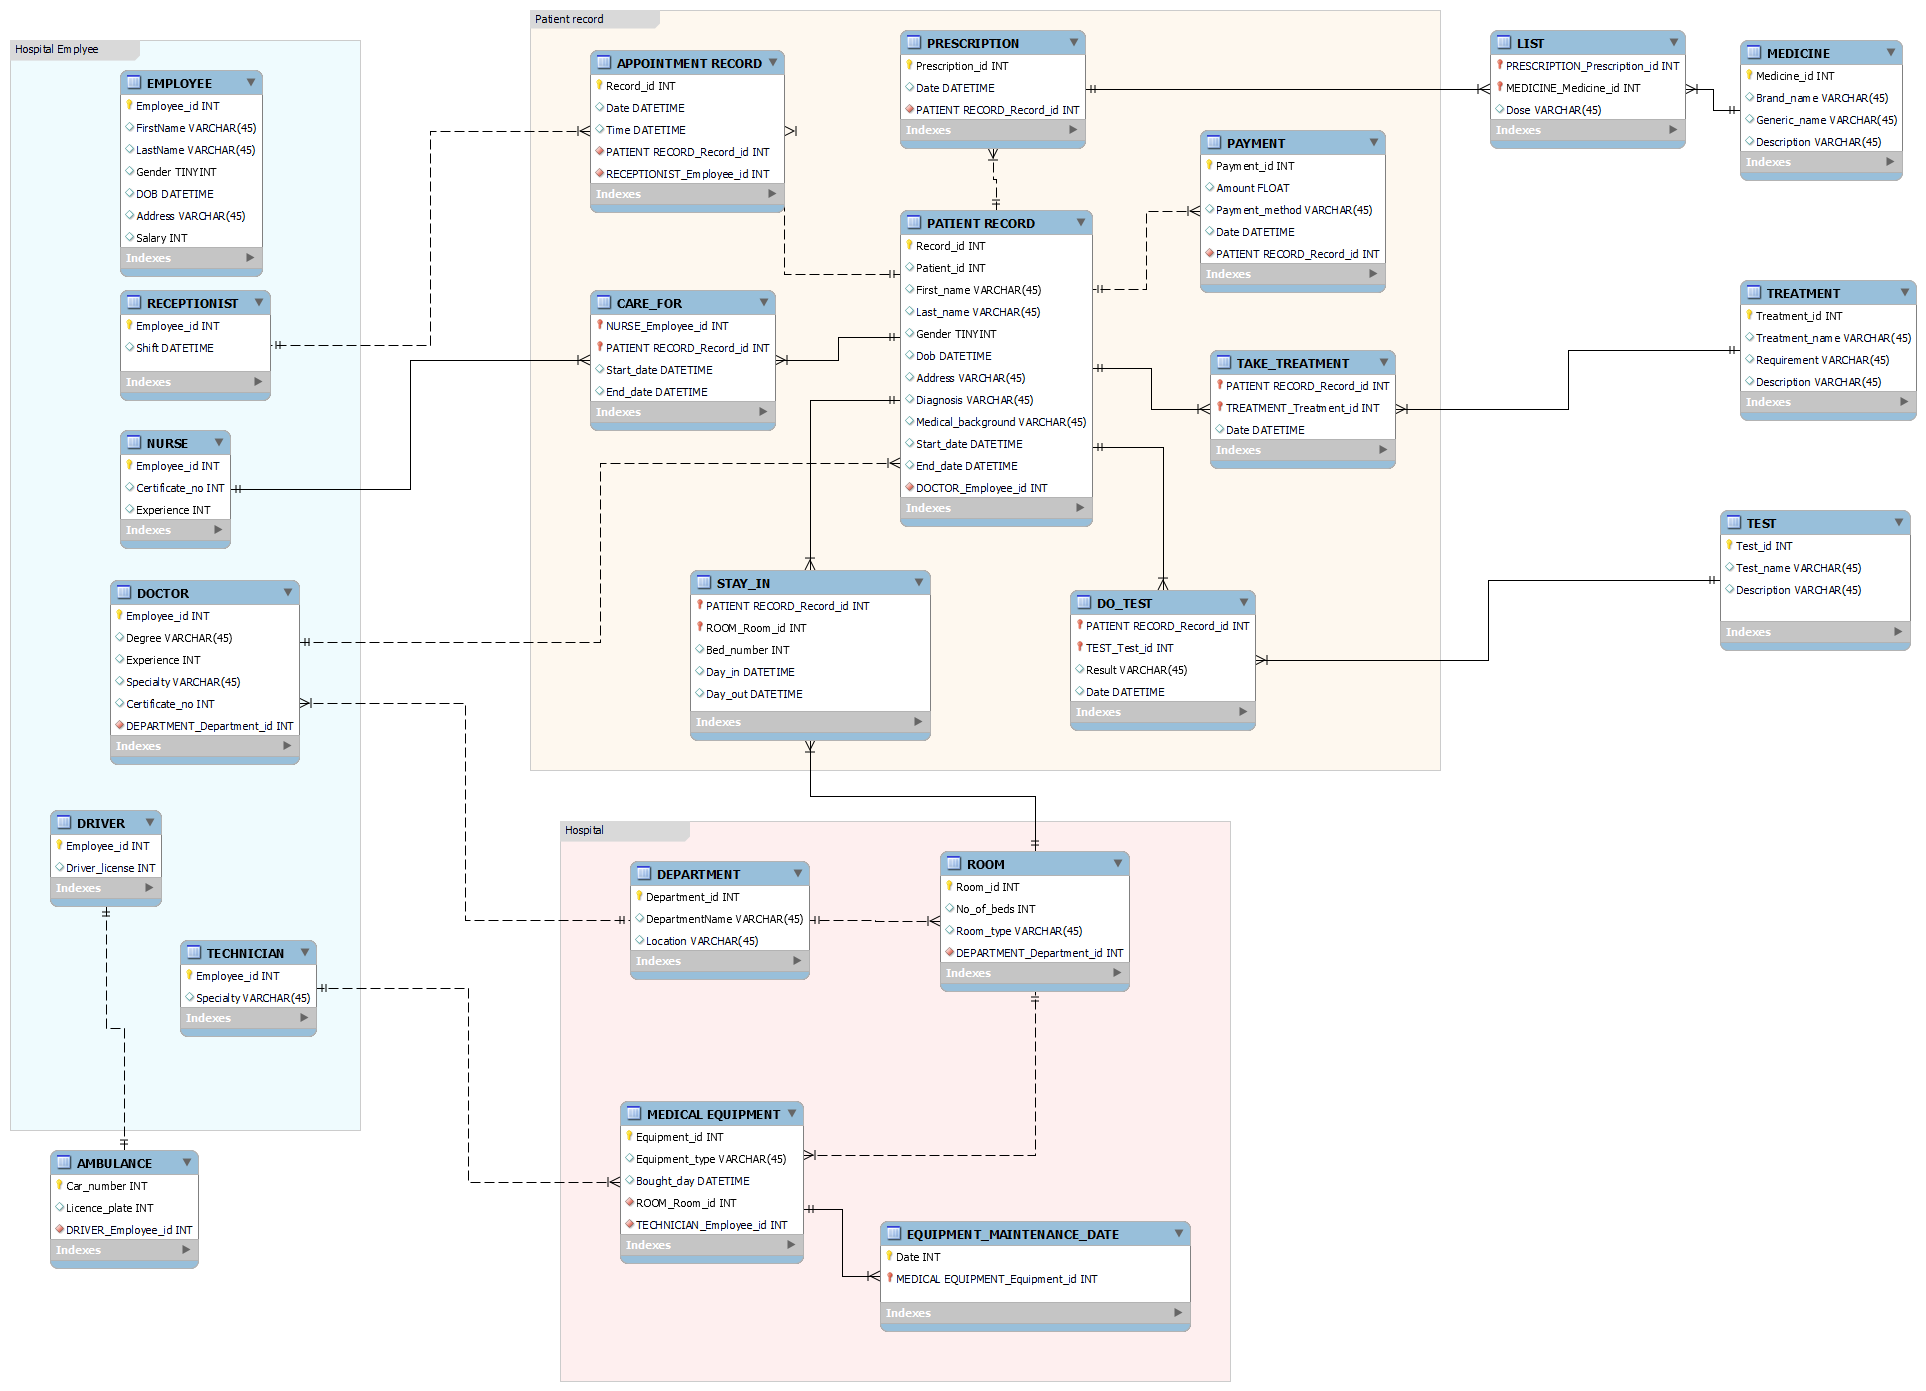
\includegraphics[width=0.9\textwidth]{./assets/logical.png}\label{Logical design}
\end{figure}

You can find a high quality version of this figure at \url{https://i.imgur.com/fxAsCSQ.png}.

\subsection{Implementation}
After we have define the design for our database, we will use a feature called forward engineering in MySQL Workbench to automatically convert our design to SQL code. 

\begin{center}
    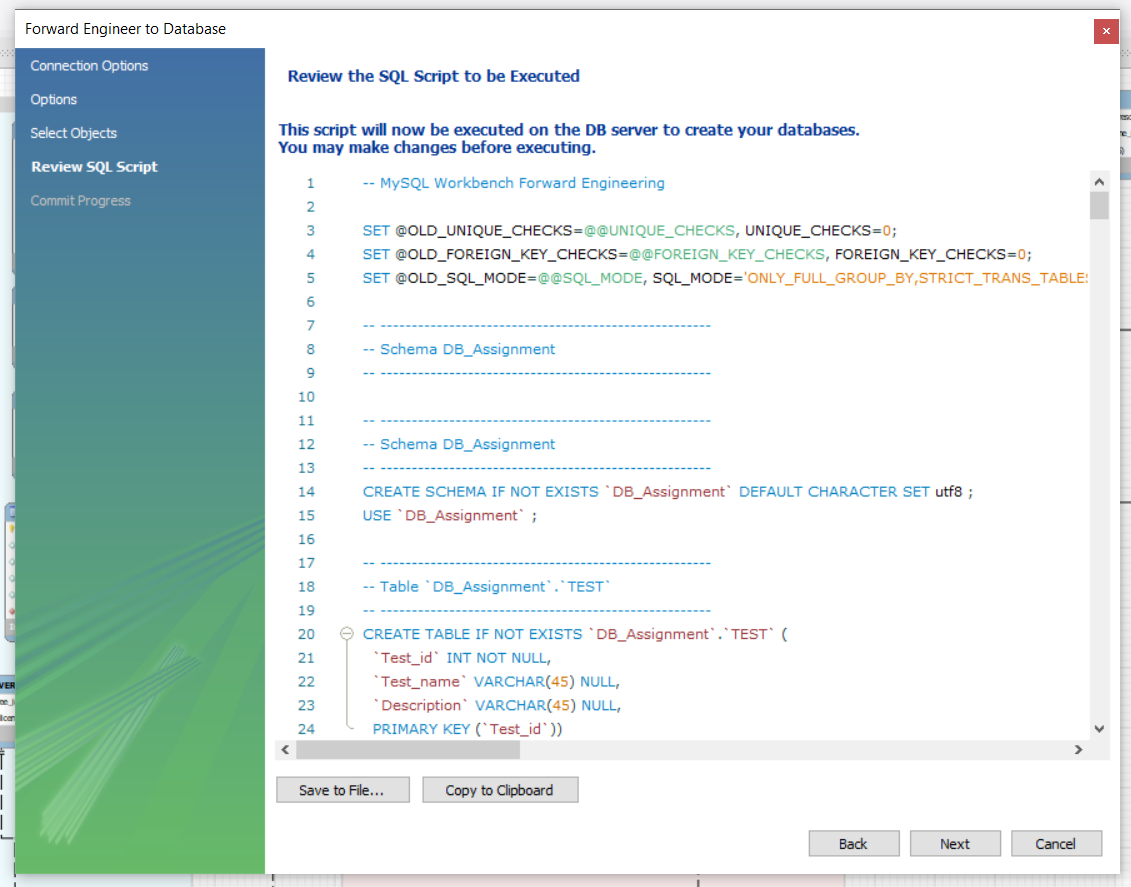
\includegraphics[width=0.9\textwidth]{assets/step1.new.png}
\end{center}

After reviewing the code, we click the ``Next'' button and receive a successfully compiled message which means that there are no errors in the code. 

\begin{center}
    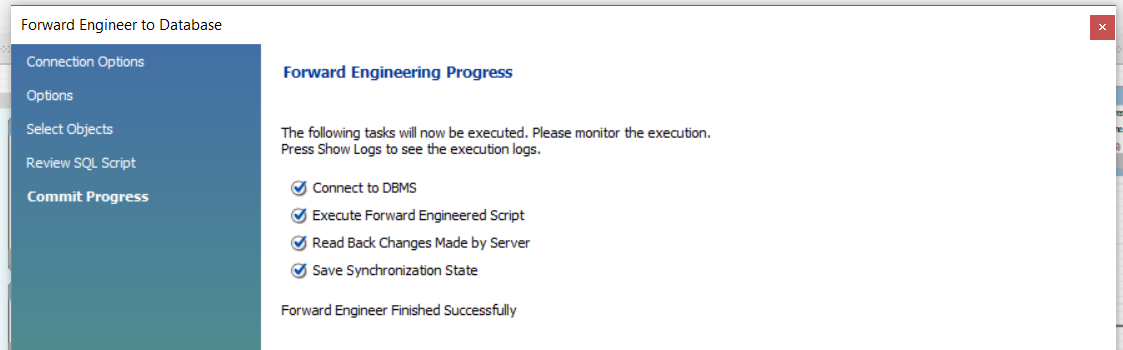
\includegraphics[width=0.9\textwidth]{assets/step2.new.png}
\end{center}

Our database is now ready to be used.

\begin{comment}
\newpage

Finally, our database is ready to be used.
\begin{center}
    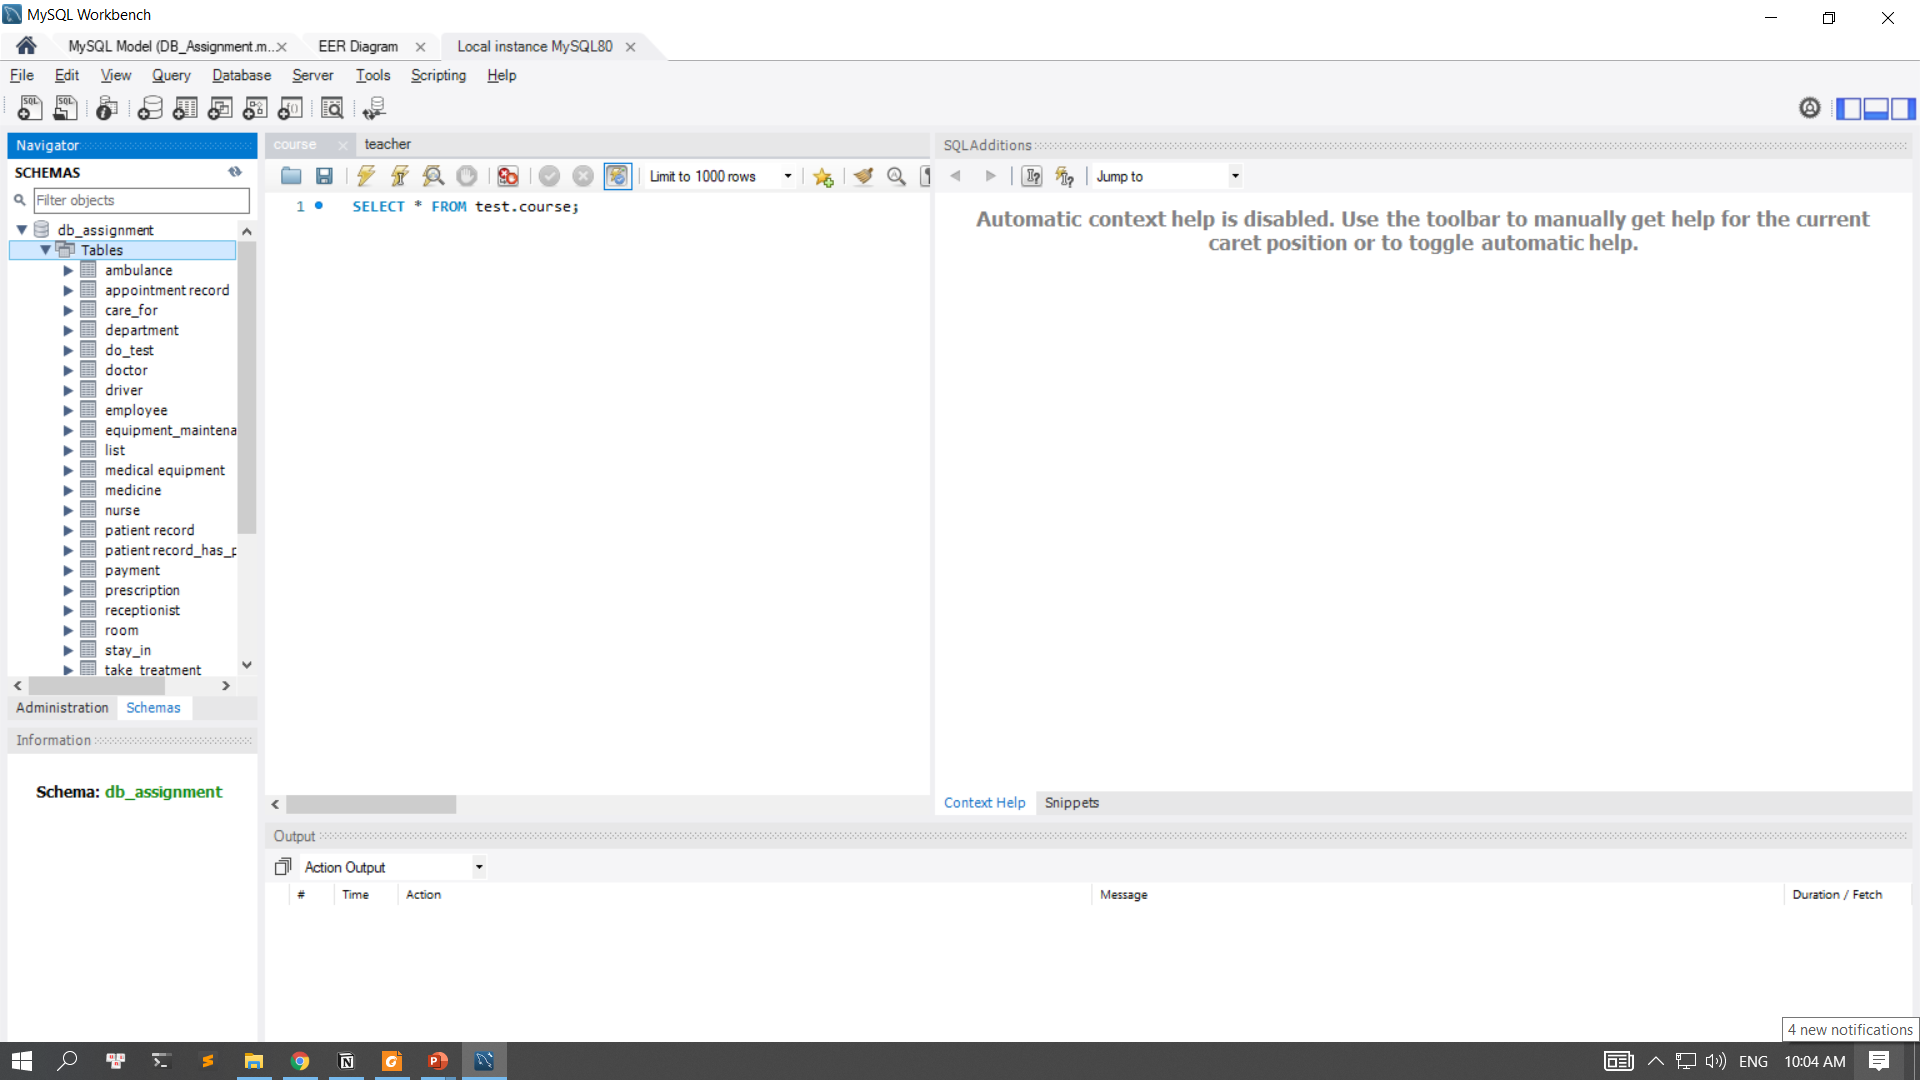
\includegraphics[width=0.9\textwidth]{assets/step3.png}
\end{center}
\end{comment}

\newpage

\section{Conclusion}
For this assignment, we have examined the hospital management system and tried to build a database for it. Regarding the requirements, the biggest difficulty we faced was the complexity of the hospital system, because a hospital have many employees types and each of them has specific role in their job. Moreover, the main purpose of a hospital management system is to record the patient medical record. Therefore, our system is built around the information stored for a patient. We also have gone through many database designing steps, including conceptual design, logical design, physical design and implementation. However, in the physical design part, we have only listed the data type constraint until now and left it there for the next assignment.
\end{document}
